\section{Data Observation: A Pilot Study on the Stress-buffering Effect of School-Scheduled Positive Events}
\label{sec:obs}
\paragraph{Microblogs} Microblogs of students from Taicang High School were collected from January 1, 2014, to September 1, 2017. 
We filtered out 121 active students out of over 500 students according to their posting frequency 
and collected their microblogs throughout their whole high school career. 
In total, 27,346 microblogs were collected in this study, 
where each student post an average of 226 microblogs, and maximum of 1,421 microblogs and a minimum of 102 microblogs. 
To protect the privacy, all the usernames were anonymized during the experiment. 

\paragraph{Scheduled events} The list of weekly scheduled school events, 
with a detailed description of the event (grade and exact start and end time), 
were collected from the school's official website\footnote{http://stg.tcedu.com.cn/col/col82722/index.html} 
from February 1, 2014 to August 1 2017. 
There were 126 stressor events and 75 positive events in total. 
Examples of positive scheduled and stressor events in high school life are listed in Table~\ref{tab:example}. 
There were 2-3 stressor events and 1-2 positive events scheduled per month in the current study. 
Figure~\ref{fig:example} shows three examples of a student's stress fluctuations around three midterm exams, 
where a positive event \emph{campus art festival} was scheduled ahead of the first exam (\emph{example a}), 
a positive event \emph{holiday} occurred after the second exam (\emph{example b}), 
and no positive scheduled event was found near the third exam (\emph{example c}). 


\begin{table}[H]
\caption{\small{Examples of school-scheduled positive and stressor events.}}
\label{tab:example}
\resizebox{.45\textwidth}{9mm}{
\small{
\begin{tabular}{cccc}
\toprule
Type & Date	& Content	& Grade	\\
\midrule
stressor event & 2017/4/16 & first day of the mid-term exam & grades 1 and 2\\
positive event & 2016/11/5 & campus art festival & grades 1, 2, and 3\\
\bottomrule
\end{tabular}
}
}
\end{table}

\begin{figure}[H]
\centering
\includegraphics[width=\linewidth]{figs/exampleWave.eps}
\caption{\small{Examples of school-scheduled positive events, stressor events, and a student's stress fluctuations}}
\label{fig:example}
\end{figure}

To further observe the effect of positive events on stressed students, 
we collected all the stressful intervals surrounding the scheduled exams for the 121 students 
during their high school career, 
applying the interval detection method from ~\citep{Li2017Analyzing}. 
For each student, we divided all the stressful intervals into two sets:
1) In the original sets, stress was caused by a stressor event, lasting for a period, and no other intervention (namely, a positive event) occurred. We called the set of such stressful intervals \textbf{SI}; 
2) In the other comparative sets, the stressful interval was impacted by a positive event. 
We called the set of such stressful intervals \textbf{U-SI}. 
Thus, the difference under the two situations (sets) could be seen as the stress-buffering effect 
induced by the positive event. 
We identified 518 exam-related stressful intervals (SI) 
and 259 stressful intervals impacted by four typical positive scheduled events (U-SI)
('practical activity', 'New Year party', 'holiday', 'sporting event') from the students' microblogs.
Six measures for the above two conditions were considered:
the \emph{accumulated value of stress}, the \emph{average value of stress} (per day),  the \emph{maximal value of stress} (per day),
the \emph{RMS value of stress},
the \emph{frequency of academic topic words}, and the \emph{ratio of academic stress among all types of stress}.
Since our target was to track the impact of positive events for students under stress,
based on previous research~\cite{XueUbicomp13},
we detected the stress level (ranging from 0 to 5) for each post.
For each student,
the stress value per day was aggregated by calculating the average amount of stress from all the posts. 
Examples of academic-related keywords are listed in Table \ref{tab:studyWords}. 
The average value of each measure over all eligible slides was calculated. 

\begin{table}[H]
\centering
\caption{\small{Examples of academic-related keywords.}}
\label{tab:studyWords}
\small{
\begin{tabular}{c}
\toprule
exam, fail, review, score, test paper, rank, pass, math, chemistry\\
homework, regress, fall behind, tension, stressed out, physics,\\
nervous, mistake, question, puzzle, difficult, lesson, careless\\
\bottomrule
\end{tabular}
}
\end{table}

\paragraph{Results}
As shown in Figure~\ref{fig:frequencyBar}, 
comparing each measure of scheduled exam intervals under the two situations 
(1) existing positive neighbouring events (U-SI) and 2) no neighbouring positive scheduled events (SI)), 
we found that students 
with exams and positive neighbouring events appeared exhibited less stress intensity
(78.13\% reduction in average stress, 95.58\%  reduction in cumulative stress, and 57.20\%  reduction in maximal stress)
and more stable stress fluctuations (47.93\% reduction in the RMS values of stress). 
Furthermore, the frequency of academic topic words (see Table \ref{tab:studyWords} for examples) 
and the ratio of academic stress in each interval were calculated. 
Most students talked less about exams when positive events occurred nearby with lower frequency (84.65\% reduction) and lower ratio (89.53\% reduction).
The statistical results show clues about the impact of positive scheduled events, 
which is consistent with psychological theory ~\citep{Cohen1984Positive, Cohen2010Positive, Needles1990Positive},
indicating the reliability and feasibility of the microblog dataset. 
However,
this observation is based on specific scheduled events,
and cannot satisfy the need for automatic, timely, and continuous perception of the stress-buffering process.
Therefore we propose a framework to automatically detect positive events and their impact intervals. 
Based on this framework, 
the relationship between the impact of automatically extracted positive events
and adolecents' microblogging characteristics will be discussed. 

\begin{figure}[h]
\centering
\includegraphics[width=\linewidth]{figs/barUSI.eps}
\caption{\small{
Comparing average stress value for all students during exam intervals in two situations: 
1) intervals affected by positive neighboring events (U-SI) and 2) no positive events occurred (SI). 
}}
\label{fig:frequencyBar}
\end{figure}

\begin{figure}[h]
\centering
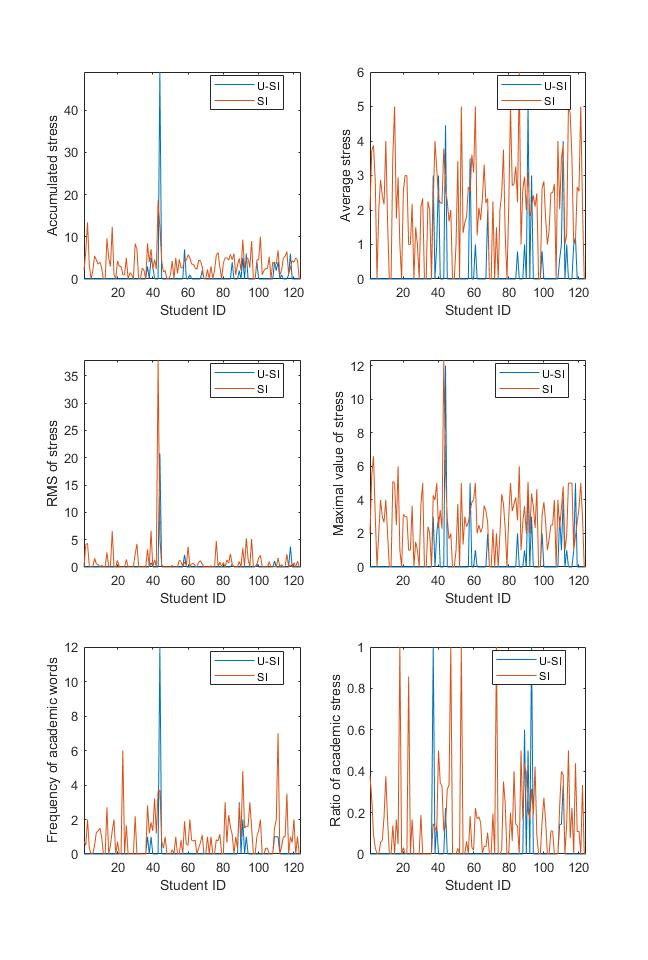
\includegraphics[width=\linewidth]{figs/activity.eps}
\caption{\small{Comparing students' stress fluctuations during exam intervals in the SI and U-SI sets.}} 
\label{fig:frequency}
\end{figure}